\section{S3}
	\subsection{Context}
	The purpose of S3, as a data storage, is used to store all files, and these files include unformatted and uncleaned data and results integrated into analytics tool. S3 gains any types of data and format data from the user and then move them to other services in Amazon platform.
        
	\subsection{Composition}
	\begin{itemize}
		\item \textbf{Buckets:} bucket is a basic container used to store objects in S3.\cite{z1}
		\item \textbf{Objects:} Objects are the fundamental entities stored in S3, and it consists of object data and metadata. The role of metadata is to store set of name-value pairs that describe the object.\cite{z1}
		\item \textbf{Keys:} each object has the unique identifier and which is called “key”. In order to ensure uniqueness of each object, the combination of a bucket, key and version ID is used to identify each object in S3.\cite{z1}
	\end{itemize}

	\subsection{Interaction}
    S3 need to upload data to analytics and send data to database, thus S3 will interact with the Data Pipeline, and then complete data transforming between different compute and storage services according to the application on data pipeline. On the other hand, the developer needs to program some functions for S3, thus S3 will interact with AWS Lambda. The role of AWS Lambda is to run code for all backed services on this platform.
    
	\subsection{Algorithm}
    The AWS SDK supports several programming languages to develop S3 by programming. The programming languages cover Java, .NET, Ruby, Python and PHP. On the other AWS SDK also provide many API for these programming languages. Take an instance with Java, the developer can utilize low-level API to implement create, update, and delete operations that apply to buckets and objects in S3.\cite{z2} 

 \section{AWS SDK for Python}
	\subsection{Context}
    The role of AWS SDK for Python is to complete all operations for data from S3 such as integrating data, parsing data and transferring data. These operations can ensure consistency and normalization of data which will be moved to the database.  
        
	\subsection{Dependency}
    This tool is not completely independent from others because the Python script must be compiled on a service. Another Amazon Web Service EC2 as the cloud-computing platform can help the developer to compile it. 
    
	\subsection{Interaction}
    AWS SDK for Python must interact with other entities. There are two reasons. One is this portion needs to receive data from other services. Second reason is the results should be exported to other services after data parsed by the Python script.

	\subsection{Algorithm}
    The core concept of AWS SDK for Python is to help developers creating one or more applications related Amazon services like S3 and DynamoDB. Boto 3 is the AWS SDK for Python and it is able to provide enough methods to solve some general problems between these services.
    
	\begin{itemize}
	\item \textbf{Accessing S3:} 
	The purpose of accessing S3 service is to gain data we want to process from it. S3 as a data storage stores all source files, so accessing S3 service is the first step in our project. The Boto 3 provides higher-level resources for S3. Then, we need to get a specific bucket in an S3 resource. There is an example showing how to access S3 service and bucket into it.\\
	\begin{lstlisting}[language=Python, caption=Accessing S3 example\cite{z4}]
		import boto3
		
		# Get the S3 service resource.
		s3 = boto3.resource('s3')
		
		# Access the bucket ‘mybucket’ into S3
		bucket = s3.Bucket('mybucket')
	\end{lstlisting}	
	
	\item\textbf{Accessing DynamoDB:}
	The purpose of accessing DynamoDB is the results must be imported to a table into DynamoDB. The basic idea to access DynamoDB is similar to access S3. We need to access a specific table after we gain DyanmoDB resources. There is still an example of them:\\
	\begin{lstlisting}[language=Python, caption=Accessing DynamoDB\cite{z4}]
		import boto3
		
		# Get the DynamoDB service resource.
		dynamodb = boto3.resource('dynamodb')

		# Access the table ‘users’ into DynamoDB
		table = dynamodb.Table('users')
	\end{lstlisting}
	\end{itemize}
       
\section{Data Pipeline}
	\subsection{Context}
    The product relates to a number of different compute and storage services thus function of AWS Data Pipeline is to help user efficiently and massively move data among these services.
     
     \subsection{Composition}
     \textbf{Data node:} entity of data source in the pipeline, and attributes of it consist of name, locations, and formats\cite{z5}. 
     
     \noindent\textbf{Activity:} activity represents methods to transform data such as moving data from one location to another. 
     
     \noindent\textbf{Schedule:} each activity has own schedule for operating data
     
     \noindent\textbf{Resources:} entity that implements activities when they are scheduled 
     
	\subsection{Dependency}
	Data Pipeline must depend on other services because the main goal of it is to transform data from other data sources. On the other hand, the activities are extensible, so the developer is allowed to run custom scripts to implement more combinations.
     
    \subsection{Structure}
	The following diagram represents a complete structure of the Data Pipeline. 

    \begin{figure}[H]
        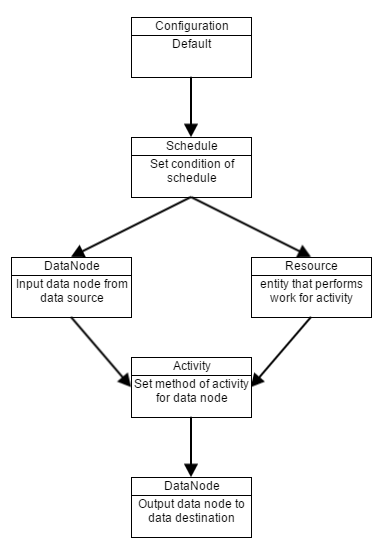
\includegraphics[width=10cm, height=14cm]{data_pipeline.png}
        \centering
        \caption{Complete structure of Data Pipeline}
    \end{figure}
    
	\subsection{Interaction}
	AWS provides management console to create a data pipeline directly. The developer can set the data source and data destination, and then the new data pipeline will automatically make  a connection between these two locations.  
    
	\subsection{Algorithm}
	In this product, the locations are S3 and DynamoDB for data pipeline, thus all of algorithms must be associated to these two services. AWS Data Pipeline supports \textbf{S3DataNode} and \textbf{DynamoDBDataNode}. The  object example of \textbf{S3dataNode} is

	\begin{lstlisting}[language=Java, caption=S3 Data Node example\cite{z6}]
        {
            "id" : "OutputData",
            "type" : "S3DataNode",
            "schedule" : { "ref" : "CopyPeriod" },
            "filePath" : "s3://myBucket/#{@scheduledStartTime}.csv"
        }
	\end{lstlisting}
	And the object example of \textbf{DynamoDBDataNode} is 
	\begin{lstlisting}[language=Java, caption=DynamoDB Data Node example\cite{z7}]
        {
            "id" : "MyDynamoDBTable",
            "type" : "DynamoDBDataNode",
            "schedule" : { "ref" : "CopyPeriod" },
            "tableName" : "adEvents",
            "precondition" : { "ref" : "Ready" }
        }
	\end{lstlisting}

	\noindent In term of algorithm of activity, AWS Data pipeline provides several general activities to accommodate common scenarios. These activities include \textbf{CopyActivity}, \textbf{HiveActivity}, \textbf{PigActivity}, etc.\\ 
    
    \noindent Resource is used to make these activities work on data node. The AWS Data Pipeline supports two kinds of resources: EC2 and EMR. The concept of \textbf{Ec2Resource} is to use EC2 instance to perform the activity but \textbf{EmrCluster} is to use EMR cluster to perform the activity. 


